\documentclass{article}
\usepackage[textwidth=170mm, textheight=230mm, inner=15mm, top=5mm, bottom=20mm]{geometry}
\usepackage[normalem]{ulem}
\usepackage[utf8]{inputenc}
\usepackage{physics}
\usepackage{scrextend}
\KOMAoption{fontsize}{11pt}
\PassOptionsToPackage{defaults=hu-min}{magyar.ldf}
\usepackage[magyar]{babel}
\usepackage{amsmath, amsthm,amssymb,paralist,array, ellipsis, graphicx, float, relsize}

\begin{document}
\renewcommand{\labelitemi}{\textbullet}
\def\R{\mathbb{R}}
\def\N{\mathbb{N}}
\def\Z{\mathbb{Z}}
\def\C{\mathbb{C}}
\def\rtr{\R\to\R}
\def\ab{[a;b]}
\def\intab{\int\limits_{a}^{b}}
\begin{center}
	{\Large\textbf{Numerikus Módszerek 2. B szakirány}}\\[0.2cm]	
	2. ZH-n kért elméleti kérdések	
\end{center}
{\small A kidolgozást \textsc{Bauer Bence} készítette \textsc{Németh Zsolt} előadásai alapján.}\\
\begin{enumerate}
	\setcounter{enumi}{29}
	\item\textbf{Definiálja a B-spline-okat (a definícióban szereplő jelölések értelmezését is adja meg).}\\[0.1cm]
	Az $f:\rtr$ \textit{függvény tartója} következo valós számhalmaz
	\begin{center}
		$supp(f):=\overline{x\in\R:f(x)\neq0}$
	\end{center}
	$\Omega_\infty:=\{...,x_{-n},...,x_{-1},x_0,x_1,..,x_n,..\}$ alappontrendszer \\[0.2cm]
	$S_l(\Omega_\infty):$ az $\Omega_\infty$ alappontrendszeren értelmezett $l$-edfokú spline-ok halmaza.\\[0.2cm]
	A $B_{l,k}\in S_l(\Omega_\infty)$ spline-okat \textit{B-spline-oknak} nevezzük, ha:
	\begin{itemize}
		\item $B_{l,k}(x)\geq0\quad(\forall x\in\R)$
		\item $supp(B_{l,k})$ minimális
		\item $\sum\limits_{k\in\Z}B_{l,k}(x)\equiv1\quad(\forall x\in\R)$
	\end{itemize}
	\item\textbf{Írja fel a 0-fokú és 1-fokú B-spline-ok képleteit és ábrázolja is őket.}\\[0.1cm]
	$l=0$ esetben a B-spline:\\[0.2cm]
	$\displaystyle B_{0,k}(x)= 
	\left\{
	\begin{gathered}
	\quad 1\quad:\quad\text{ha }x\in[x_k;x_{k+1})\hspace{5.7cm} \\
	\quad 0\quad:\quad\text{különben}\hspace{7cm}
	\end{gathered}\right.$\\
	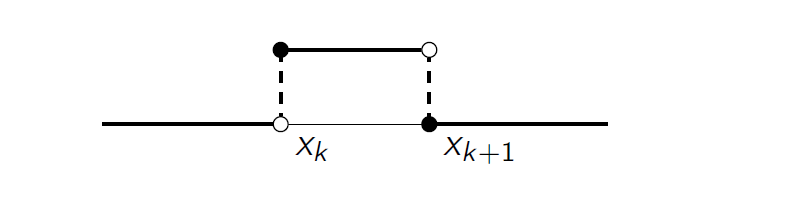
\includegraphics[width=10cm]{images/bspline0.png}\\
	$l=1$ esetben a B-spline:\\[0.2cm]
	$\displaystyle B_{1,k}(x)= 
	\left\{
	\begin{gathered}
	\quad\frac{x-x_k}{x_{k+1}-x_k}\quad:\quad\text{ha }x\in[x_k;x_{k+1})\hspace{5.7cm}
	\\[0.2cm]\quad\frac{x_{k+2}-x}{x_{k+2}-x_{k+1}}\quad:\quad\text{ha }x\in[x_{k+1};x_{k+2})\hspace{5.7cm} \\
	\quad 0\quad:\quad\text{különben}\hspace{5.4cm}
	\end{gathered}\right.$\\
	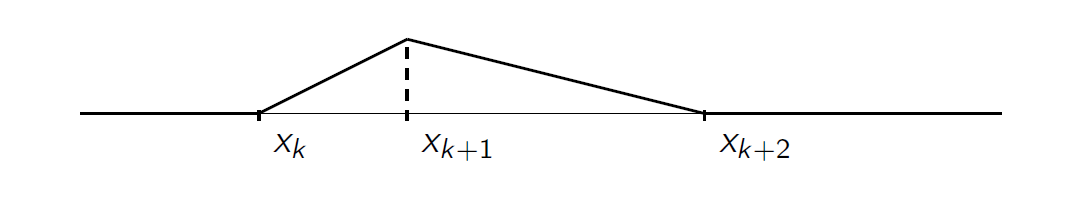
\includegraphics[width=10cm]{images/bspline1.png}
	\item\textbf{Milyen rekurziót tanult B-spline-okra?}\\[0.1cm]
	{\Large $B_{l,k}(x)=\frac{x-x_k}{x_{k+l}-x_k}\cdot B_{l-1,k}(x)+ \frac{x_{k+l+1}-x}{x_{k+l+1}-x_{k+1}}\cdot B_{l-1,k+1}(x)\quad(x\in\R)$}
	\item\textbf{Milyen tételt tanult spline előállítására B-spline-ok felhasználásával?}\\[0.1cm]
	{\Large $\forall S\in S_l(\Omega_\infty):\exists c_k\in\R(k\in\N):S(x)=
	\sum\limits_{k=-\infty}^{\infty}c_k\cdot B_{l,k}(x)\\[0.1cm]
	\forall S\in S_l(\Omega_n):\exists c_{-l},...,c_{n-1}\in\R:S(x)=
	\sum\limits_{k=-l}^{n-1}c_k\cdot B_{l,k}(x)$}
	\newpage
	\item\textbf{Egyenletes felosztás esetén milyen alakú a B-spline bázisban felírt másodfokú spline együtthatóinak egyenletrendszere?}\\[0.1cm]
	$l=2$ esetben a B-spline a $h_k\equiv h$ esetben\\[0.1cm]
	$\displaystyle B_{2,k}(x)= 
	\left\{
	\begin{gathered}
	(x-x_k)^2,\hspace{4.5cm}\text{ha }x\in[x_k;x_{k+1}]\hspace{5.7cm}
	\\[0.1cm]h^2+2h(x-x_{k+1})-2(x-x_{k+1})^2,\hspace{0.8cm}\text{ha }x\in[x_{k+1};x_{k+2}]\hspace{5.7cm}
	\\[0.1cm](x_{k+3}-x)^2,\hspace{4.5cm}\text{ha }x\in[x_{k+2};x_{k+3}]\hspace{5.7cm}\\
	\quad 0,\hspace{5.8cm}\text{különben}\hspace{8cm}
	\end{gathered}\right.$\\
	\item\textbf{Egyenletes felosztás esetén milyen alakú a B-spline bázisban felírt harmadfokú spline együtthatóinak egyenletrendszere?}\\[0.1cm]
	$l=3$ esetben a B-spline a $h_k\equiv h$ esetben\\[0.1cm]
	$\displaystyle B_{3,k}(x)=\frac{1}{6h^3}\cdot
	\left\{
	\begin{gathered}
	(x-x_k)^3,\hspace{6.6cm}\text{ha }x\in[x_k;x_{k+1}]\hspace{5.7cm}
	\\[0.1cm]h^3+3h^2(x-x_{k+1})+3h(x-x_{k+1})^2-3(x-x_{k+1})^3,\text{ha }x\in[x_{k+1};x_{k+2}]\hspace{5.7cm}
	\\[0.1cm]h^3+3h^2(x_{k+3}-x)+3h(x_{k+3}-x)^2-3(x_{k+3}-x)^3,\text{ha }x\in[x_{k+2};x_{k+3}]\hspace{5.7cm}
	\\[0.1cm](x_{k+4}-x)^3,\hspace{6.6cm}\text{ha }x\in[x_{k+3};x_{k+4}]\hspace{5.7cm}\\
	\quad 0,\hspace{7.5cm}\text{különben}\hspace{7cm}
	\end{gathered}\right.$\\
	\item\textbf{Milyen hibabecslést tanult 1-fokú spline interpolációra?}\\[0.1cm]
	Ha $f\in C^2\ab$ és $S\in S_1(\Omega_n)$ lineáris interpolációs spline, akkor\\[0.2cm]
	{\Large $||f-S||_\infty\leq\frac{1}{8}h^2\cdot||f''||_\infty,\quad$ ahol
	$h:=\max\limits_{i=1}^{n}\abs{h_k}$}
	\item\textbf{Milyen hibabecslést tanult 3-fokú spline interpolációra?}\\[0.1cm]
	Ha $f\in C^4\ab$ és $S\in S_3(\Omega_n)$ köbös interpolációs spline 
	Hermite-peremfeltétellel, akkor\\[0.2cm]
	{\Large $||f-S||_\infty\leq\frac{5}{384}h^4\cdot||f^{(4)}||_\infty\\[0.2cm]
	||f'-S'||_\infty\leq\frac{1}{24}h^3\cdot||f^{(4)}||_\infty\\[0.2cm]
	||f''-S''||_\infty\leq\frac{3}{8}h^2\cdot||f^{(4)}||_\infty,\quad$ ahol
	$h:=\max\limits_{i=1}^{n}\abs{h_k}$}
	\item\textbf{Mit nevezünk mátrix szinguláris felbontásának, mik a szinguláris értékek?}\\[0.1cm]
	Tetszőleges $A\in\C^{m\cross n}$ esetén $\exists U\in\C^{m\cross m},V\in\C^{n\cross n}$
	unitér mátrix és $D\in\C^{m\cross n}$,\\[0.1cm]particionálva $D=
	\begin{bmatrix} \sum & 0 \\ 0 & 0 \end{bmatrix}$, hogy $A=UDV^*$\\[0.1cm]
	ahol $\sum=diag(\sigma_1,...,\sigma_r),r=$rang(A) és $\sigma_1\geq...\geq\sigma_r>0$
	\\[0.3cm] A szinguláris felbontásbeli $\sigma_1,...,\sigma_r>0$ értékeket az
	\textit{A szinguláris értékeinek} nevezzük.\\[0.1cm]
	{\Large $\sigma_i=\sqrt{\lambda_i(A^*A)}>0,\quad(i=1,...,r)$}
	\item\textbf{Hogyan jellemzhető lineáris transzformáció a szinguláris felbontás segítségével?}\\[0.1cm]
	Tetszőleges $A\in\C^{m\cross n}$ mátrix és $\sigma_1\geq...\geq\sigma_r>0$ szinguláris
	értékek esetén rang(A)$=r$,\\[0.1cm]továbbá ker(A)$=span\{u_1,...,u_r\}$ és Im(A)
	$=span\{v_{r+1},...,v_n\}$
	\newpage
	\item\textbf{Mit mond ki az Eckart–Young tétel?}\\[0.1cm]
	Ha rang(A)$=r$, akkor a $k$ rangú legjobb közelítése eloállítható a szinguláris felbontásból\\[0.1cm]
	{\Large $A_k=\sum\limits_{i=1}^{k}\sigma_iu_iv_i^T$}\\[0.1cm]
	ahol $\sigma_i$ az $i$. szinguláris értéket, $u_i$ és $v_i$ a bal és jobb szinguláris
	vektort jelöli. Ez a közelítés a 2-es és a Frobenius normában is a legjobb, a hibák:
	\\[0.1cm]{\Large $||A-A_k||_F=\sqrt{\sum\limits_{i=k+1}^{r}\sigma_i^2}\quad\quad
	||A-A_k||_2=\sigma_{k+1}$}
	\item\textbf{Definiálja mátrix általánosított inverzét.}\\[0.1cm]
	Az $A\in\C^{m\cross n}$ mátrix \textit{Moore-Penrose-féle általánosított
	inverze} az $A^+\in\C^{n\cross m}$ mátrix, ha
	\begin{itemize}
		\item $AA^+$ önadjungált,
		\item $A^+A$ önadjungált,
		\item $AA^+A=A$,
		\item $A^+AA^+=A^+$
	\end{itemize}
	\item\textbf{Hogyan áll elő az általánosított inverz az általános esetben?}\\[0.1cm]
	A $D\in\C^{m\cross n}$ diagonális mátrix általánosított inverze a $D^+\in\C^{n\cross m}$
	diagonális mátrix, ahol\\[0.1cm]$d_{ii}^+=\frac{1}{d_{ii}}$, ha $d_{ii}\neq0$,
	különben 0 az értéke
	\\[0.1cm]A szinguláris felbontás felhasználásával az $A\in\C^{m\cross n}$ mátrix
	általánosított inverze a következő alakban állítható elő: $\quad A^+=VD^+U^*$, ahol
	$D^+\in\C^{n\cross m}$
	\item\textbf{Hogyan áll elő az általánosított inverz a teljes rangú esetekben?}\\[0.1cm]
	Túlhatározott eset:\\[0.1cm]
	Legyen $A\in\C^{m\cross n},m>n$ és $r=$rang(A)$=n$. Ekkor:$\quad A^+=(A^*A)^{-1}A^*$
	\\[0.1cm]Alulhatározott eset:\\[0.1cm]
	Legyen $A\in\C^{m\cross n},m<n$ és $r=$rang(A)$=m$. Ekkor:$\quad A^+=A^*(AA^*)^{-1}$
	\item\textbf{Mit nevezünk LER általánosított megoldásának?}\\[0.1cm]
	Legyen $A\in\C^{m\cross n},b\in\C^m$, ekkor az $x^+:=A^+b\in\C^n$ vektort az
	$Ax=b$ \textit{LER általánosított megoldásának} nevezzük.
	\item\textbf{Ismertesse az általánosított inverz approximációs tulajdonságait.}
	\begin{itemize}
		\item $||Ax-b||_2\geq||Ax^+-b||_2,\quad\forall x\in\C^n$
		\item $H:=\{x\in\C^n|\text{  }||Ax-b||_2=||Ax^+-b||_2\}$, akkor\\[0.1cm]
		$||x^+||_2<||x||_2\quad\forall x\in\C^n,\quad x\neq x^+$
	\end{itemize}
	\item\textbf{Ismertesse a legkisebb négyzetek módszerének feladatát.}\\[0.1cm]
	Adottak az $x_1,...,x_N\in\ab$ különbözo alappontok, $y_1,...,y_N\in\R$
	függvényértékek vagy mérési eredmények. Olyan $p_n\in P_n$ polinomot keresünk
	($n+1\leq N$, általában $N\gg n$), melyre\\[0.1cm]
	{\Large $\sum\limits_{i=1}^{N}(y_i-p_n(x_i))^2$ minimális}\\[0.1cm]
	A $p_n$ polinomot négyzetesen legjobban közelítő polinomnak nevezzük.
	\item\textbf{Írja fel a Gauss-féle normálegyeneleteket.}\\[0.1cm]
	{\Large $a^+=A^+y=(A^TA)^{-1}\cdot A^Ty\quad\Leftrightarrow\quad A^TA\cdot a^+=A^Ty$}
	\newpage
	\item\textbf{Mit nevezünk interpolációs kvadratúra formulának?}
	\begin{itemize}
		\item A $\sum\limits_{k=0}^{n}A_kf(x_k)$ formulát \textit{kvadratúra formulának} nevezzük.
		\item A kvadratúra formula \textit{interpolációs típusú}, ha
		$A_k=\intab l_k(x)dx\quad(k=0,...,n)$
	\end{itemize}
	\item\textbf{Ismertesse az interpolációs kvadratúrákra tanult pontossági tételt.}\\[0.1cm]
	$\forall f\in P_n$-re $\intab f(x)dx=\sum\limits_{k=0}^{n}A_kf(x_k)\quad\Leftrightarrow
	\quad A_k=\intab l_k(x)dx\quad(k=0,...,n)$
	\item\textbf{Adja meg a kvadratúra formulák 3 főbb típusát.}
	\begin{itemize}
		\item\textbf{Newton-Cotes típus:} Az $\{x_i:i=0,...,n\}$ alappontok egyenletes
		felosztású pontok $\ab$-n
		\item\textbf{Csebisev típus:} $A_k\equiv A\quad(k=0,...,n)$
		\item\textbf{Gauss típus:} maximális $(2n+1)$ fokszámig pontos formulák.
	\end{itemize}
	\item\textbf{Definiálja a zárt illetve nyílt Newton–Cotes formulákat.}\\[0.1cm]
	Nyílt formulák (Ny(n)): $a$ és $b$ \textit{nem} alappont\\[0.1cm]
	$h=\frac{b-a}{n+2},\text{  }k=1,...,n+1$, azaz $x_0=a+h$, $x_n=b-h$\\[0.2cm]
	Zárt formulák (Z(n)): $a$ és $b$ alappont\\[0.1cm]
	$h=\frac{b-a}{n},\text{ és }k=0,...,n$, azaz $x_0=a$, $x_n=b$
	\item\textbf{Írja fel az érintő, trapéz és Simpson formulák képleteit.}
	\begin{itemize}
		\item Érintő (Ny(0)): $\intab f\approx(b-a)\cdot f\big(\frac{a+b}{2}\big)=:E(f)$
		\item Trapéz (Z(1)): $\intab f\approx\frac{b-a}{2}\cdot(f(a)+f(b))=:T(f)$
		\item Simpson (Z(2)): $\intab f\approx\frac{b-a}{6}\cdot(f(a)+4\big(
		\frac{a+b}{2}+f(b)\big))=:S(f)$
	\end{itemize}
	\item\textbf{Adjon hibabecslést az érintő, trapéz és Simpson formulákhoz.}
	\begin{itemize}
		\item Érintő: Ha $f\in C^2\ab$, ekkor $\exists\eta\in\ab:\intab f-E(f)=
		\frac{(b-a)^3}{24}\cdot f''(\eta)$
		\item Trapéz: Ha $f\in C^2\ab$, ekkor $\exists\eta\in\ab:\intab f-T(f)=
		-\frac{(b-a)^3}{12}\cdot f''(\eta)$
		\item Simpson: Ha $f\in C^4\ab$, ekkor $\exists\eta\in\ab:\intab f-S(f)=
		-\frac{(b-a)^5}{2880}\cdot f^{(4)}(\eta)$
	\end{itemize}
	\item\textbf{Mit nevezünk összetett trapéz formulának? Adja meg a hibabecslését.}\\[0.1cm]
	$\intab f\approx\frac{b-a}{2m}\cdot\bigg(f(a)+2\sum\limits_{k=1}^{m-1}
	f(x_k)+f(b)\bigg)=:T_m(f)$\\[0.3cm]Hibabecslés:\\[0.1cm]
	{\Large Ha $f\in C^2\ab$, ekkor $\exists\eta\in\ab:\intab f-T_m(f)=-\frac{(b-a)^3}{12m^2}\cdot f''(\eta)$}
	\newpage
	\item\textbf{Mit nevezünk összetett Simpson formulának? Adja meg a hibabecslését.}\\[0.1cm]
	$S_m(f):=\frac{b-a}{3m}\cdot\bigg(f(a)+4\sum\limits_{k=1}^{\frac{m}{2}}
	f(x_{2k}-1)+2\sum\limits_{k=1}^{\frac{m}{2}-1}f(x_{2k})+f(b)\bigg)\\[0.1cm]
	\intab f\approx S_m(f)$\\[0.3cm]Hibabecslés:\\[0.1cm]
	{\Large Ha $f\in C^4\ab$, ekkor $\exists\eta\in\ab:\intab f-S_m(f)=
	-\frac{(b-a)^5}{180m^4}\cdot f^{(4)}(\eta)$}
\end{enumerate}
\end{document}